\section{Evaluation}
\label{res_overview}
\begin{figure*}[ht]
    \centering
    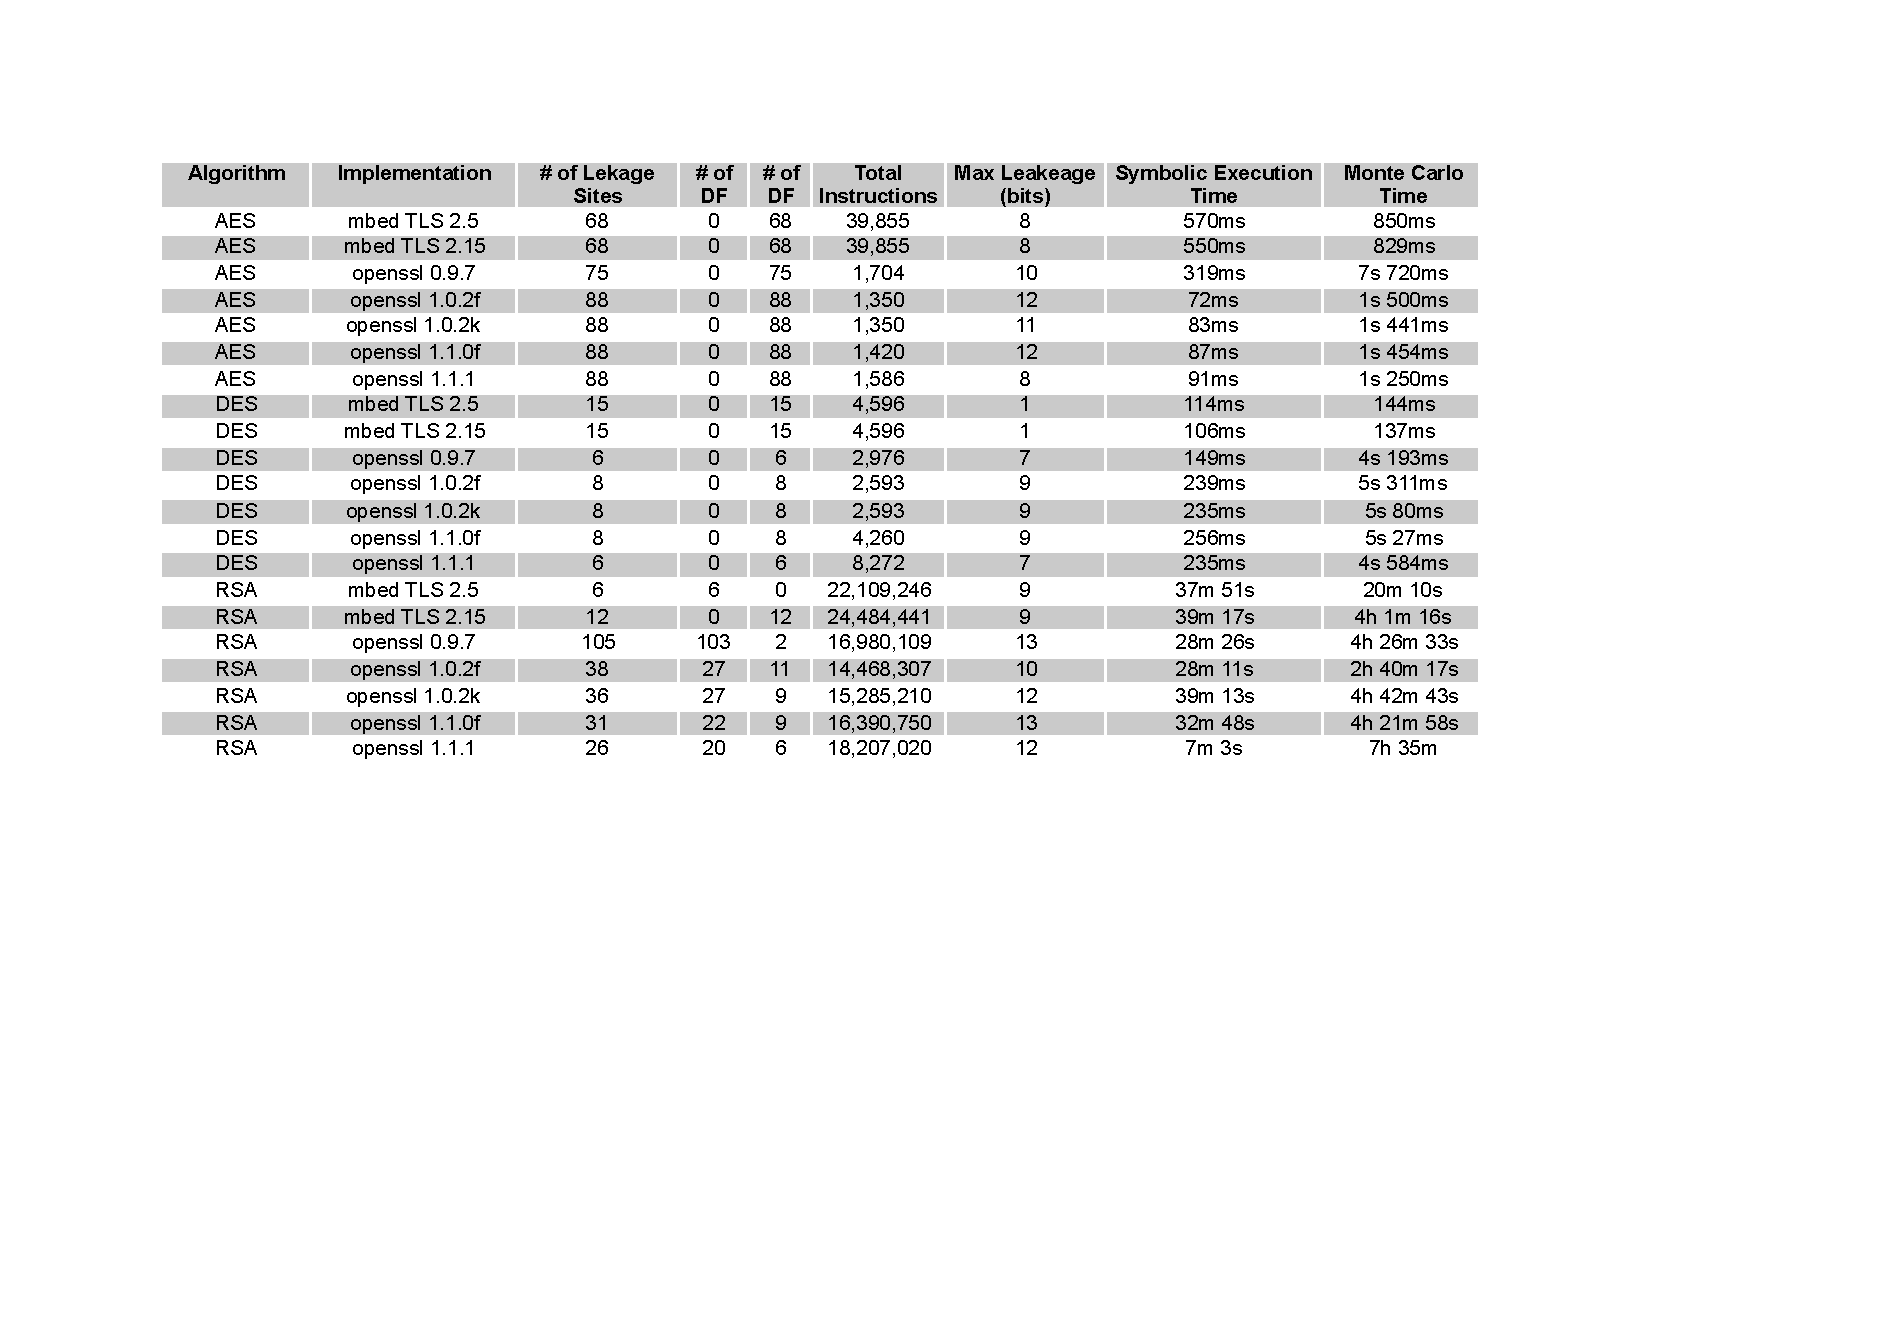
\includegraphics[width=\columnwidth]{./figures/Result.pdf}
    \caption{Result}
    \label{fig:Test}
\end{figure*}
We evaluate \tool{} with the real-world crypto libraries and non-crypto libraries. 
For crypto libraries, we choose OpenSSL, mbedTLS and NaCl. 
OpenSSL and mbedTLS are the two most commonly used
crypto libraries in today's software. NaCl (pronounced "salt") is a 
new software libreary for encryption, decryption and signatures, etc.
NaCl is designed to have no data flow from secrets to load address and no data 
flow from secrets to branch conditions. Therefore, NaCl should have no leakages
under our attack model. 

For non-crypto libraries, we study libjepg, GTK, and wget.
JPEG is a commonly used lossy image c ompression standard, and
libjpeg is a popular library for handling the JPEG image data
format. Previously, researchers have introduced controlled-channel
attacks, which allow attackers to ret rieve outlines of JPEG images
from applications. We also study GTK and wget with \tool{}. GTK 
is a widely used cross-platform toolkit for creating graphical user
interfaces. And wget is free software that can retrieve information
via HTTPS, HTTP, and FTP.

We build the source code into 32-bit x86 Linux executables with the 
GCC 8.0 on Ubuntu 14.04. Although our tool can
work on stripped binaries, we use symbol information to track
back leakage sites in the source code. We use Intel Pin version 3.7 
to record the execution trace. We run our experiments on a 2.90GHz
Intel Xeon(R) E5-2690 CPU with 128GB memory.
During the evaluation, we are interested in the following two
aspects:
\begin{enumerate}
    
    \item  Can \tool{} precisely
    report the number of leaked bits in open source libraries?
    \item  Recent work has reported a number
    of side-channel vulnerabilities in open source libraries. 
    Is the number of leaked bits reported by \tool{} useful to justify 
    the sensitive level of side-channel vulnerabilities?
   
\end{enumerate}

\subsection{Evaluation Result Overview}
In this section, we present an overview of the evaluation result. 
\tool{} find xx leakages in total from real-world cryptosystems source libraries.
 Among the xx leak points, xx of them are leaked due
to secret-dependent control-flow transfers and xx of them are leaked 
due to secret-dependent memory accesses. 

For crypto libraries, \tool{} finds that secret-dependent memory accesses 
cause most leakages. 
\tool{} also identifies that most side-channel vulnerabilities 
leak very little information in practice, which confirms our initial
assumptions. 
However, we do find some sensitive leakages. 
Some of them have been confirmed by existing research that those 
vulnerabilities can be exploited to realize real attacks. 

All the symmetric key implementations in OpenSSL and mbedTLS all yield
significant leakages due to the implementation of the lookup table
to speed up the computation. Every leakages found during the evaluation
belongs to the type of secret-dependent memory accesses. We believe that
the secret-dependent control-flow transfers have been widely studied in
the past few years, and developers have patched most of those leakages. 
One method to address the leakage is to use bit-slicing. We will analyse
the corresponding countermeasure in the following sections.

\tool{} find several leakage sites for the implementation of DES in OpenSSL.
Each leakage can leak one bit of information from one byte. Also, our tool
confirms those leakages are independent, so the total leaked information leakage
is 8 bits. We check the source code and find the least significant
bit in each byte is used for the parity. Therefore, \tool{} can confirm
that even the key length of DES is 64 bits. However, only 56 bits of the 
DES key is valid. 



\subsection{Information Leakage Quantification}
\subsection{Analysis of Software Countermeasures}
\subsubsection{Bit-slicing}
\subsubsection{Scatter and Gather}
\subsection{Case Studies}
\subsubsection{libjpeg}

